%
% Copyright (c) 2011-2013, fortiss GmbH.
% Licensed under the Apache License, Version 2.0.
% 
% Use, modification and distribution are subject to the terms specified
% in the accompanying license file LICENSE.txt located at the root directory
% of this software distribution. A copy is available at
% http://chromosome.fortiss.org/.
%
% This file is part of CHROMOSOME.
%
% $Id$
%

% =================================================================
\section{Example 4: Integrating External Nodes (20 minutes)}
\label{sec:example_lonelyNode}
% =================================================================

In previous examples, we have generated the code for nodes that have been modeled within the same deployment model in \xmt.
These nodes were hence known a priori and the generated code is based on this knowledge.
This allows to establish all connections from the start.

However, this scenario does not always apply.
In case we want to add a new node to an already existing ecosystem of nodes,
the new node needs to be developed independently from current established nodes.
%
In this example, we will generate a new deployment model without having information about nodes that are already running in \xme.

For modeling the firmware of the new node called \emph{Lonely Node}, we again use \xmt.
For this purpose, we will start again the Eclipse workspace and import the deployment model
\emph{deploymentLonelyNode.xmn} located at \verb|<XME_ROOT>/examples/sensorMonitor| (compare Figure~\ref{fig:xmt_deploymentLonely}).
%
You should note that if you have already imported all models in previous example,
the \emph{lonely node} will be already imported in your workspace.

\begin{figure}[htpb]
	\centering
	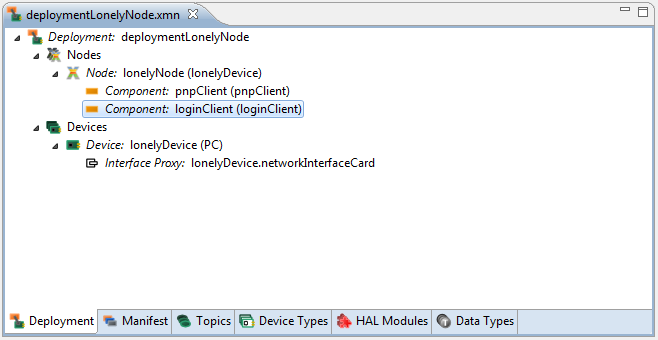
\includegraphics[scale=0.5]{figures/xmt_deploymentLonely.png}
	\caption{Lonely Node deployment model.}
	\label{fig:xmt_deploymentLonely}
\end{figure}

We assume here that the code for running the \emph{monitorNode}, \emph{sensorNode} and \emph{emptyNode} is already generated and compiled.
In case that this is not yet the case, please follow the steps explained in the example in Section~\ref{sec:example_xmt} before continuing.

% ~~~~~~~~~~~~~~~~~~~~~~~~~~~~~~~~~~~~~~~~~~~~~~~~~~~~~~~~~~~~~~~~~~
\subsection{Overview of lonelyNode}
% ~~~~~~~~~~~~~~~~~~~~~~~~~~~~~~~~~~~~~~~~~~~~~~~~~~~~~~~~~~~~~~~~~~

For the deployment model of \emph{lonely node}, we already use generated components which are part of \xmt, such as \emph{loginClient} and \emph{pnpClient}.
These two components play the following roles in this scenario:

\begin{itemize}
	\item The \emph{loginClient} component establishes a connection with the \emph{Login Manager}
		(here running on the \emph{monitorNode}) in order to register the \emph{lonelyNode}.
	
	\item After login is completed, the \emph{pnpClient} component announces the application components
		running on the \emph{lonelyNode} to the \emph{Plug and Play Manager} (also running on the \emph{monitorNode}).
		\emph{Plug and Play Manager} will then establish the required communication routes.
\end{itemize}
%
For more information about how the login and plug~\&~play infrastructure works, please refer to Section~\ref{sec:example_pnp}.

As it is generated from \xmt, the lonely node contains the code for starting an \xme instance of this node.
However, as the lonely node does not contain any information about configurations of already running nodes --
for example it does not know where the \emph{Login Manager} is located --
it needs to discover the network configuration for using the login and plug~\&~play services.

The login operation is performed using broadcasting of a login request and the plug~\&~play operation is completed using the configuration
received from the login response, which contains the interface address where the \emph{Plug and Play Manager} is listening to \emph{component instance manifests}.

Now let's generate the code for \emph{lonelyNode}:
just like in the previous example, right-click on the \emph{Deployment: deploymentLonelyNode} in the deployment model
and click on \emph{Generate Application Code...}~--~see Figure~\ref{fig:xmt_deploymentLonely_generate}.
Confirm the code generation dialog accordingly.

\begin{figure}[ht]
	\centering
	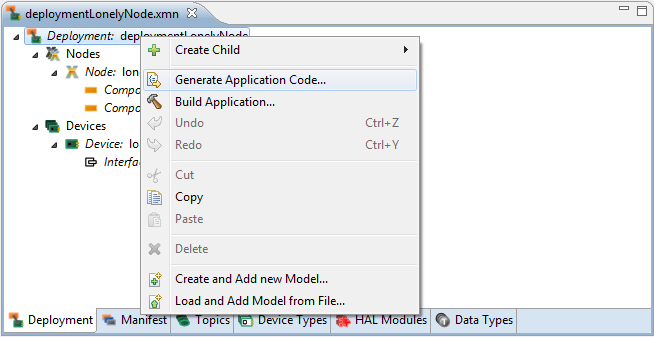
\includegraphics[scale=0.5]{figures/xmt_deploymentLonely_generate.png}
	\caption{Generation of application code for \emph{lonelyNode}.}
	\label{fig:xmt_deploymentLonely_generate}
\end{figure}

In order to compile the generated code, right-click on the \emph{Deployment: deploymentLonelyNode}
and select \emph{Build Application...}~--~see Figure~\ref{fig:xmt_deploymentLonely_build}.

\begin{figure}[ht]
	\centering
	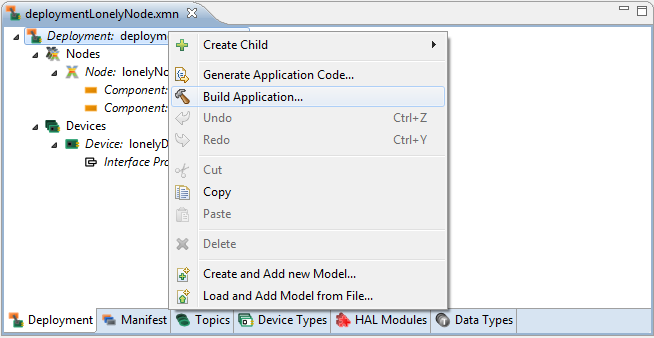
\includegraphics[scale=0.5]{figures/xmt_deploymentLonely_build.png}
	\caption{Build of application code for \emph{lonelynode}.}
	\label{fig:xmt_deploymentLonely_build}
\end{figure}

In the build window, select \emph{lonelyNode} and check \emph{Generate Build System} and \emph{Compile}
as shown on Figure~\ref{fig:xmt_deploymentLonely_buildWindow}.
Then click \emph{OK}.

\begin{figure}[ht]
	\centering
	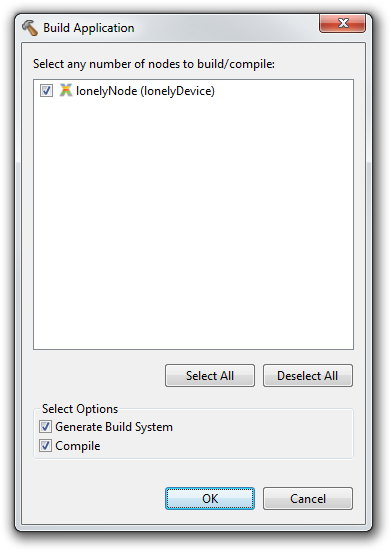
\includegraphics[scale=0.75]{figures/xmt_deploymentLonely_buildWindow.png}
	\caption{XMT build options for lonely node.}
	\label{fig:xmt_deploymentLonely_buildWindow}
\end{figure}

The output of the build is created in the \verb|build/lonelyNode| folder inside the \emph{sensorMonitor} project in the workspace.

% ~~~~~~~~~~~~~~~~~~~~~~~~~~~~~~~~~~~~~~~~~~~~~~~~~~~~~~~~~~~~~~~~~~
\subsection{Running the lonelyNode}
% ~~~~~~~~~~~~~~~~~~~~~~~~~~~~~~~~~~~~~~~~~~~~~~~~~~~~~~~~~~~~~~~~~~

After compilation is finished, the \emph{lonelyNode} is ready to run.
Before of running the executable, make sure that at least the node containing \emph{Login Manager} and the \emph{Plug~\&~Play Manager} is currently running.
If you followed the instructions in this tutorial, that node is the \emph{monitorNode}.

\emph{lonelyNode} includes in the manifests for deploying one \emph{sensorB} component.\footnote{%
	The pnpClient will announce any component type listed in the \emph{pluggable components} attribute of its node. For lonely node this list only contains a \emph{sensorB}.
}
To run the lonely node, just double-click on Eclipse workspace file \verb|/build/lonelyNode/target/Debug/|
\verb|lonelyNode.exe|.
%
As soon as the node is started, it should emit login requests that are handled by the \emph{Login Manager}.
After a couple of seconds, login should be complete and the component manifest exchanged.
Then, \emph{Plug and Play Manager} should update the communication routes such that
the \emph{sensorB} on \emph{lonelyNode} sends its data to the \emph{monitorB} on \emph{monitorNode}
(compare Figure~\ref{fig:example_lonelyNode}).
%

%In the case we are running all four nodes (\emph{monitorNode}, \emph{sensorNode}, \emph{emptyNode} and \emph{lonelyNode}),
%the \emph{lonelyNode} will publish sensor data to \emph{monitorNode} and in \emph{emptyNode}, and will subscribe to sensing data published by \emph{sensorNode} and \emph{emptyNode}.
%Additionally, the \emph{monitor} in \emph{lonelyNode} will receive publications produced by \emph{sensor} on \emph{lonelyNode}.

\begin{figure}[htpb]
	\centering
	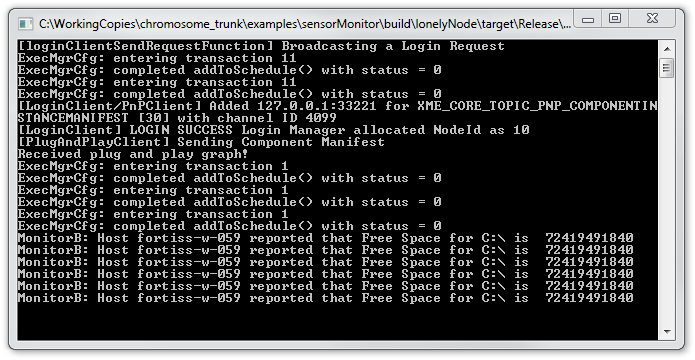
\includegraphics[scale=0.7]{figures/example_lonelyNode.png}
	\caption{Console window of \emph{lonelyNode} during login and plug~\&~play.}
	\label{fig:example_lonelyNode}
\end{figure}

% ~~~~~~~~~~~~~~~~~~~~~~~~~~~~~~~~~~~~~~~~~~~~~~~~~~~~~~~~~~~~~~~~~~
\subsection{Conclusion}
\label{sec:example_lonelyNode:conclusion}
% ~~~~~~~~~~~~~~~~~~~~~~~~~~~~~~~~~~~~~~~~~~~~~~~~~~~~~~~~~~~~~~~~~~

In this example, we have generated code for a new node which is developed completely independent from from the other nodes in the network.
The only shared specification between the nodes is the topic dictionary, which defines the structure of the data being exchanged.
%
The newly node, named \emph{lonelyNode}, completes its registration in \emph{Login Manager} component
located at \emph{monitorNode} (or any other node containing the \emph{Login Manager}),
exports its \emph{component instance manifest} to the \emph{Plug and Play Manager},
and -- in this case -- starts the components \emph{sensor} and \emph{monitor} after successful login.
%
In this example, you learned how to develop a new component from scratch, without any connection to an existing infrastructure of \xme.
